\chapter{Lecture: Binary Search Trees, BST Sort}
\href{https://ocw.mit.edu/courses/electrical-engineering-and-computer-science/6-006-introduction-to-algorithms-fall-2011/lecture-videos/lecture-5-binary-search-trees-bst-sort/}{Lecture 5} from the MIT's 
Intro to Algorithms.

Consider the runway reservation system problem. Let's assume this airport has a single runway. We are working 
on reservations for future landings. We need to reserve requests for landings time, \(t\). Add \(t\) to the set \(R\) of
landing times if no other landings are scheduled within \(k\) minutes. After the plane lands, remove from \(R\).
We will do all these operations in \(\theta(\log_2 n)\) where \(n\) is the size of the set. For this example, let \(k = 3\).
That is, \(\lvert t_i - 3\rvert\geq 3\) to insert a new \(t_i\) in set \(R\). Additionally, we cannot insert times in the past.
\begin{enumerate}
	\item The set cannot be unordered array; we cannot use binary search.
	\item With a sorted array, we can find the insertion point in order \(\theta(\log_2 n)\), \(\theta(1)\) to check \(k\)
	against \(t_{i\pm 1}\), but it will take order \(\theta(n)\) to insert and shift.
	\item With a sorted linked list, we could insert in \(\theta(1)\) but we couldn't use binary search.
	\item With heaps (min or max), an element that is \(\leq k\) of \(\geq k\) from \(t\) then \(\theta(n)\) time.
	\item Dictionaries would be \(\theta(n)\) as well.
\end{enumerate}
If we could we do fast insertion into a sorted linked list, we would be in business.

Binary search trees
\begin{figure}[h]
	\centering
	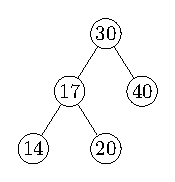
\includegraphics[width=3in]{binary_search_tree5.pdf}
	\caption{Binary Search Tree}
	\label{fig5:bst}
\end{figure}
Each node \(x\) has a key for \(x\). Unlike a heap, the BST has pointers that are parent, left, and right child of \(x\).
For all nodes \(x\), if \(y\) is in the left subtree of \(x\), then \(key(y)\leq key(x)\). If \(y\) is in the right subtree, then
\(key(y)\geq key(x)\). From a null BST, we have
\begin{enumerate}
	\item Insert \(49\)
	\item Insert \(79\) but since \(79 > 49\), we attach to the right child of \(49\)
	\item Insert \(46\) and since \(46 < 49\), we attach to the left child of \(49\)
	\item Insert \(41\) then \(41 < 49\) so go left and \(41 < 46\) so attach to the left child of \(46\)
	\item Try to insert \(42\). \(42 < 49\) so go left, \(42 < 46\) so go left, and \(42 > 41\) but not \(k\) more than \(3\)
	insertion fails.
\end{enumerate}
If \(h\) is the height of the tree, then insertion with or without the check, is done in order \(\theta(h)\) time. In BST, we
can find the min or the max by going to the left or right until leaf, respectively. These would be in \(\theta(h\).
New requirement: rank \(t\) how many planes are scheduled to land at times \(\leq t\)? How can we do this without
changing the complexity? Let's augment the BST structure. We can add another value to the node key. When we do 
insert and delete, we modify the subtree size numbers. 
\begin{figure}[h]
	\centering
	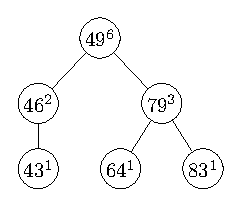
\includegraphics[width=3in]{augmented_bst5.pdf}
	\caption{With an augmented BST, we would append number of subtrees to each node.}
	\label{fig5:augmented_bst}
\end{figure}
A single node would be 1, a node with 2 children below
would be 3, and root would be the number of nodes. That is, just the number of nodes underneath parent plus
itself. What lands before \(t\) in order \(\theta(h)\) time?
\begin{enumerate}
	\item Walk down the tree to find the desired time
	\item Add in the nodes that are smaller
	\item Add in the subtree sizes to the left
\end{enumerate}
Let \(t = 79\). What is \(\leq t\)?
\begin{enumerate}
	\item \(49\) is clearly less than \(t\) so add \(1\)
	\item Move to the right but first add the sub tree sizes to the left; add \(2\)
	\item \(79\) is equal to so add \(1\)
	\item Look left and \(1\) from the subtree to left node \(64\)
\end{enumerate}
We have \(5\). See lecture 6 for how to get \(\theta(\log_2 n)\) complexity.




